\section{Results}
\label{sec:results}

The numerical results for the problem described in Section \ref{sec:requests} are reported in the following.

When not specified, the results are obtained with the following boundary conditions imposed on the structure:

\begin{table}[H]
    \centering
    \begin{tabular}{|l|c|c|c|c|}
        \hline
        ~            & $U_x$ & $U_y$ & $V_x$ & $V_y$ \\
        ~            & m     & m     & m/s   & m/s   \\
        \hline
        Bottom nodes & Fixed & Fixed & 0     & 0     \\
        Top nodes    & -     & Fixed & 1     & 0     \\
        \hline
    \end{tabular}
    \caption{Boundary conditions imposed on the structure.}
    \label{tab:boundary_conditions}
\end{table}


\paragraph{Average $\sigma_{12}(\gamma)$ for element \#1}

To answer the first question of the assignment, we have decided to consider for the computation of the average shear stress $\sigma_{12}$ just the first element of the mesh, which is the one in the bottom-left corner of the structure.
Moreover, given that $\sigma_{12}$ get computed in every Gaussian point of the element, to simplify the computation, we have decided to consider just the Gaussian point in elemental coordinates $(\eta, \xi) = (-1/\sqrt{3}, -1/\sqrt{3})$, which is the one in the bottom-left corner of the element.
This choice is justified by the fact that $\gamma$, which is the shear strain of the element, is usually referred to the bottom-left corner of the element with the hypotheses of null gradient all over the element (i.e., $\gamma_{element} = \gamma_{bottom-left} \rightarrow \gamma(x, y) = \gamma(0, 0)$).

With the hypothesis of null or almost null $\nabla \gamma$ in the element, we report in Figure \ref{fig:shear_stress_vs_strain} the shear stress $\sigma_{12}$ as a function of the shear strain $\gamma$ until $\gamma = 0.07$.

\begin{figure}[H]
    \centering

    \begin{minipage}[b]{0.45\textwidth}
        \centering
        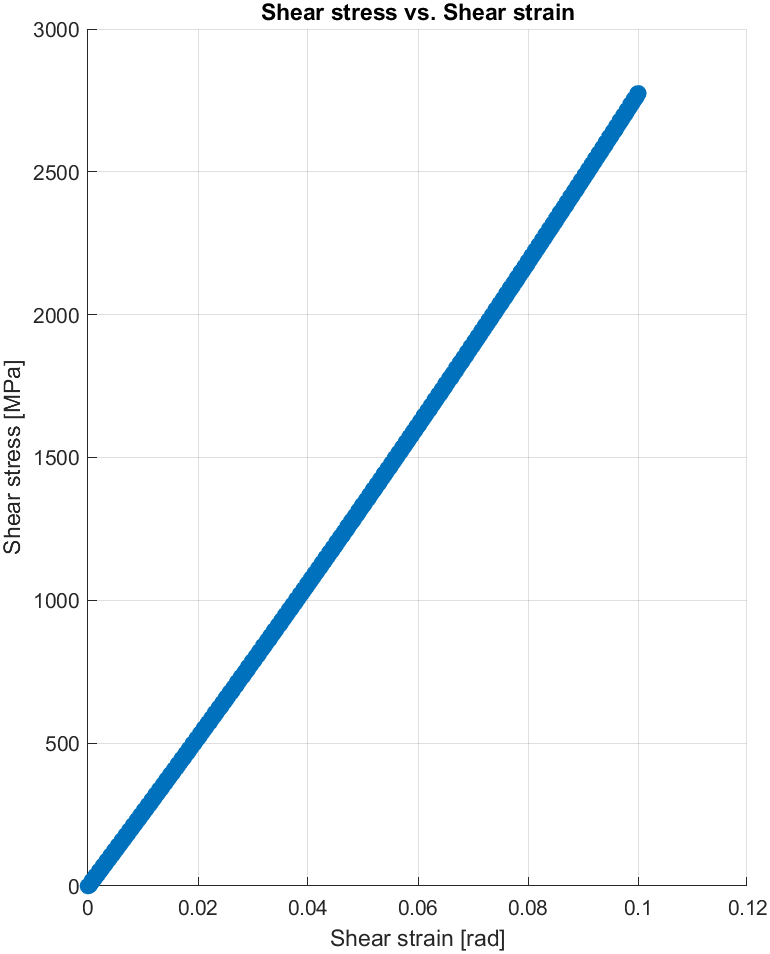
\includegraphics[width=\textwidth]{img/shear_stress_vs_strain.png}
        \caption{Average shear stress $\sigma_{12}$ as a function of the shear strain $\gamma$.}
        \label{fig:shear_stress_vs_strain}
    \end{minipage}
    %
    \hfill
    %
    \begin{minipage}[b]{0.45\textwidth}
        \centering
        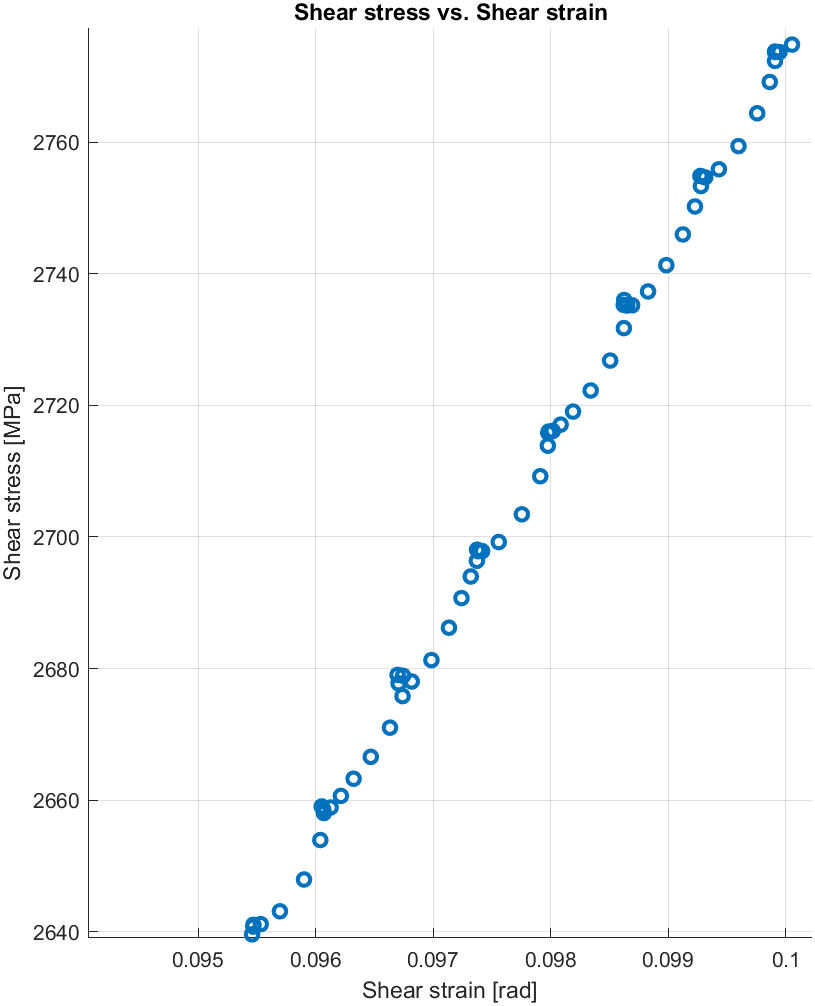
\includegraphics[width=\textwidth]{img/shear_stress_vs_strain_focus.png}
        \caption{Focus on the oscillation of the curve $\sigma_{12}(\gamma)$.}
        \label{fig:shear_stress_vs_strain_focus}
    \end{minipage}

\end{figure}

From the plot, it's clearly visible a general linear trend of the stress-strain curve, which is typical for a linear elastic material.
In particular, the curve well approximate the ideal behavior having a slope almost equal to the shear modulus $G = \frac{E}{2(1 + \nu)} = 26.923 \text{GPa}$, characteristic of the elastic region of the material.

However, because of the inertia effects and the high loading speed, the curve is not perfectly linear, and it shows some oscillations.
When the loading speed is reduced to a more realistic value, such as $v = 0.001 \text{m/s}$, the inertia effects are strongly reduced, and the oscillatory behavior of the curve is almost completely removed.


\paragraph{Initial and final positions of the structure}

In Figure \ref{fig:initial_vs_final}, we can observe the structure in both its initial configuration (shown in blue), and in its final configuration (shown in red).

\begin{figure}[H]
    \centering
    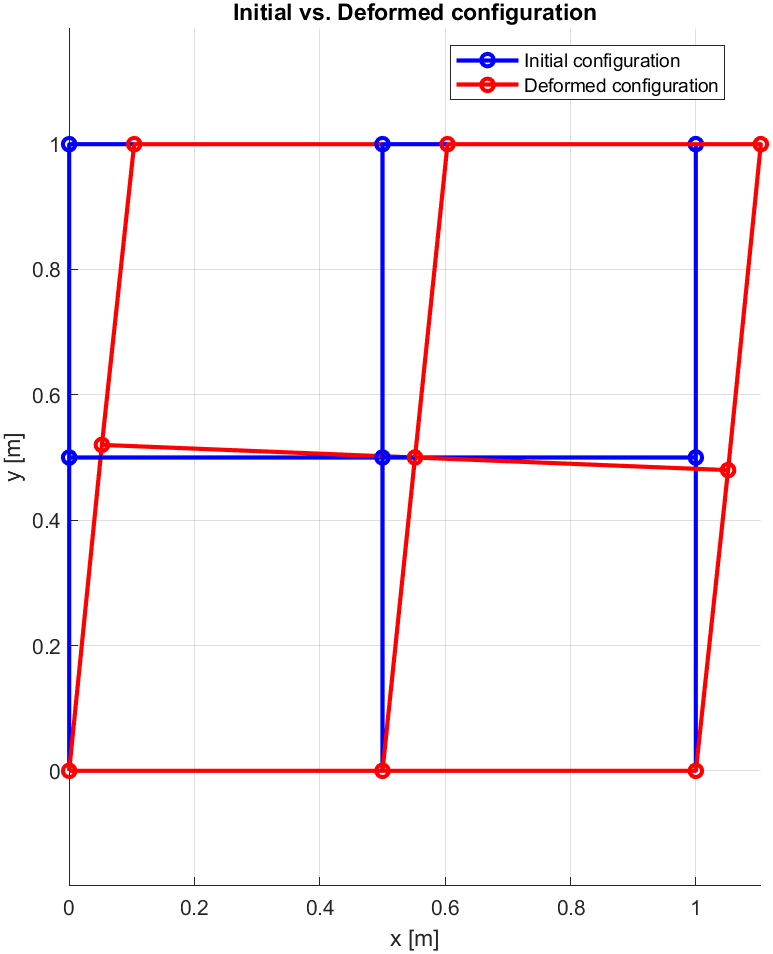
\includegraphics[width=0.5\textwidth]{img/initial_vs_final.png}
    \caption{Initial and final configurations of the structure.}
    \label{fig:initial_vs_final}
\end{figure}

The structure is deformed in the $\vec{x}$ direction, as expected, and the deformation is more pronounced in the top part of the structure where the velocity constrains is applied.
The deformation is almost linear, and the structure is not showing any sign of instability or excessive deformation.

The well known behavior of compression on the right side and tension on the left side of the lower half of the structure is clearly visible by observing the central line which is horizontal in the initial configuration and shows a clear clockwise rotation in the final configuration.


\paragraph{Computation time reduction}

Finally, a possible way to reduce the computation time when the loading speed is reduced to a more realistic value, such as $v = 0.001 \text{m/s}$, is to increase the density property of the material ($\rho$).

This choice is motivated by the fact that the time step of the simulation is usually limited by the smallest element of the mesh, which is the one that requires the smallest time step to satisfy convergence and stability conditions.
In particular:

\begin{equation}
    \Delta t = \frac{2}{\omega_{max}}
    \label{eq:time_step}
\end{equation}

where $\omega_{max}$ is the maximum frequency of the system, computable as the largest eigenvalues of the equation of motion for the element (i.e., $[M] \ddot{U} + [K] U = 0 \rightarrow det([M] \omega^2 - [K]) = 0 \rightarrow \omega_{max}$).
By solving the equation, we obtain the following expression for the time step:

\begin{equation}
    \Delta t = \frac{L_{min}}{c} = \frac{L_{min}}{\sqrt{\frac{E}{\rho}}} = \frac{L_{min}}{\sqrt{E}} \sqrt{\rho}
    \label{eq:time_step_2}
\end{equation}


where $L_{min}$ is the smallest characteristic length of the element, and $c$ is the speed of sound in the material.

From Equation \ref{eq:time_step_2}, it's clear that by increasing the density of the material, the time step of the simulation is increased as well, and the computation time is decreased.

One may wonder if the choice of increasing the density of the material may affect the results of the simulation.
For this purpose, we report in Table \ref{tab:time_step_validation} the results of the simulation for two different values of applied velocity $v_{top}$ and density $\rho$.

\begin{table}[H]
    \centering
    \begin{tabular}{|l|c|c|c|c|c|}
        \hline
        ~            & $v_{top}$ & $\rho$                  & CPU time & $U_x$  & $U_y$  \\
        ~            & m/s       & kg/m\textsuperscript{3} & s        & m      & m      \\
        \hline
        Simulation 1 & 1         & 2700                    & 9.64     & 0.5518 & 0.5000 \\
        Simulation 2 & 0.01      & 2700                    & 662.17   & 0.5518 & 0.5000 \\
        Simulation 3 & 0.01      & 27000000                & 7.68     & 0.5518 & 0.4992 \\
        \hline
    \end{tabular}
    \caption{
        Results of the simulation for different values of applied velocity $v_{top}$ and density $\rho$.
        Here $U_x$ and $U_y$ are the displacements of the central node of the structure.
        When increasing the density of the material, the external body force (gravity) is increased as well.
    }
    \label{tab:time_step_validation}
\end{table}

From Table \ref{tab:time_step_validation}, it's clear that the results of the simulation are not affected by the choice of increasing the density of the material (as long as the mesh is sufficiently fine) and that the computation time is significantly reduced by this choice.


\subsection{Effect of mesh refinement}

It's worth mentioning that the results of the simulation are affected by the choice of the mesh size.

In Figure \ref{fig:mesh_refinement}, we report the results of the simulation runned with same boundary conditions (Table \ref{tab:boundary_conditions_for_mesh_refinement}) but different mesh sizes (Table \ref{tab:mesh_sizes}).

\begin{table}[H]
    \centering
    \begin{tabular}{|l|c|c|c|c|}
        \hline
        ~            & $U_x$ & $U_y$ & $V_x$ & $V_y$ \\
        ~            & m     & m     & m/s   & m/s   \\
        \hline
        Bottom nodes & Fixed & Fixed & 0     & 0     \\
        Top nodes    & -     & Fixed & 1000  & 0     \\
        \hline
    \end{tabular}
    \caption{Boundary conditions imposed on the structure.}
    \label{tab:boundary_conditions_for_mesh_refinement}
\end{table}

\begin{table}[H]
    \centering
    \begin{tabular}{|c|c|c|}
        \hline
        \textbf{Mesh size} & \textbf{Number of elements} & \textbf{CPU time (s)} \\
        \hline
        Coarse             & 2x2                         & 0.20                  \\
        Fine               & 4x20                        & 8.58                  \\
        \hline
    \end{tabular}
    \caption{Mesh sizes and CPU time of the simulations.}
    \label{tab:mesh_sizes}
\end{table}

\begin{figure}[H]
    \centering

    \begin{minipage}[b]{0.45\textwidth}
        \centering
        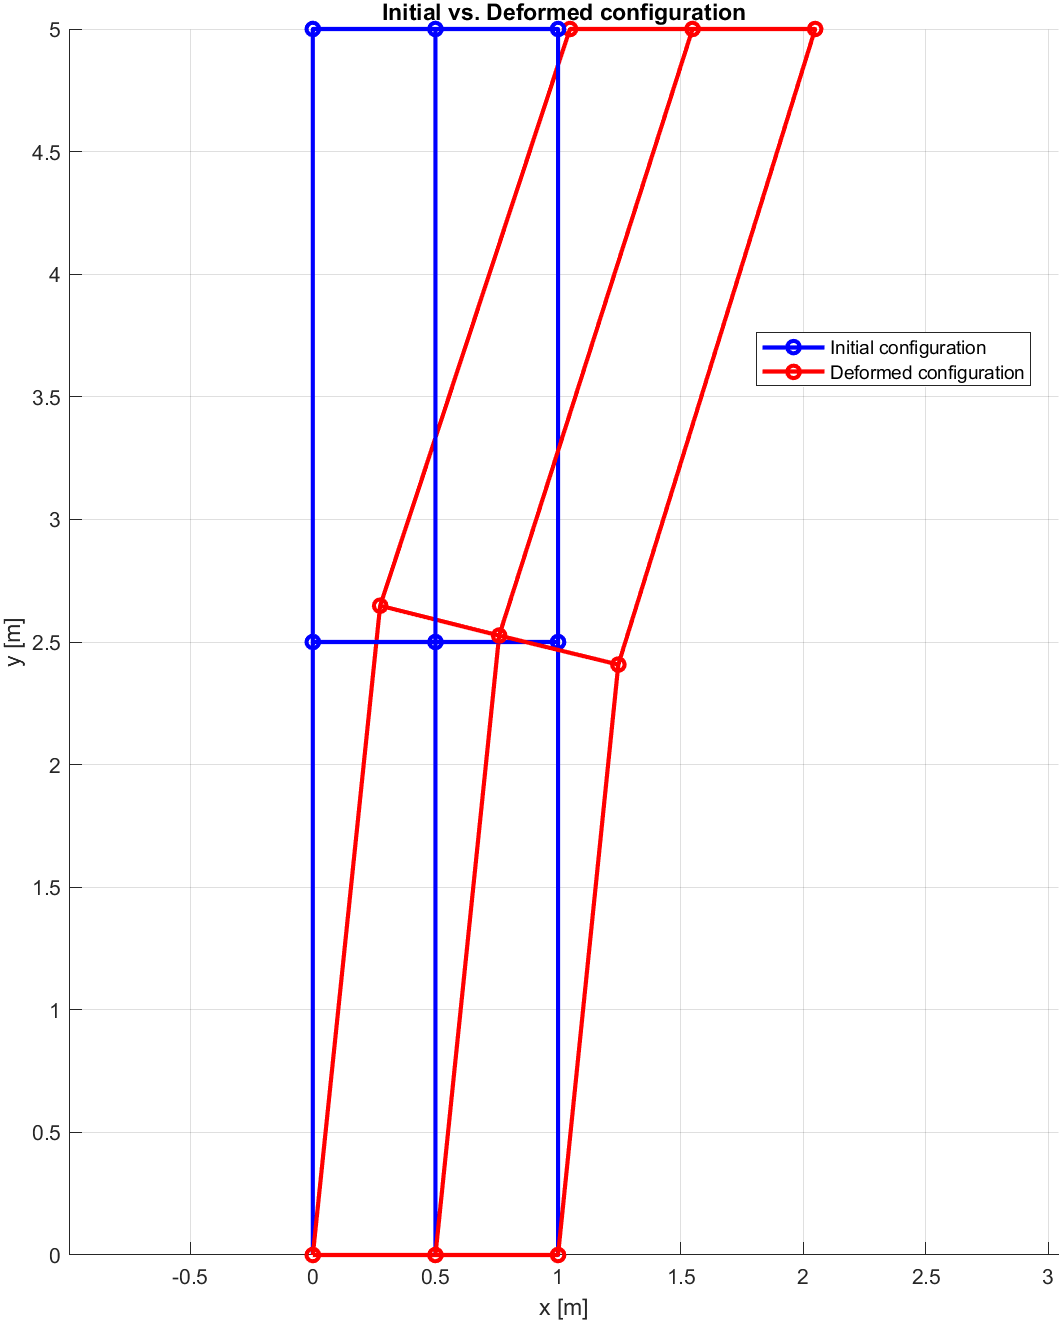
\includegraphics[width=\textwidth]{img/mesh_coarse.png}
        \caption{Coarse mesh.}
    \end{minipage}
    %
    \hfill
    %
    \begin{minipage}[b]{0.45\textwidth}
        \centering
        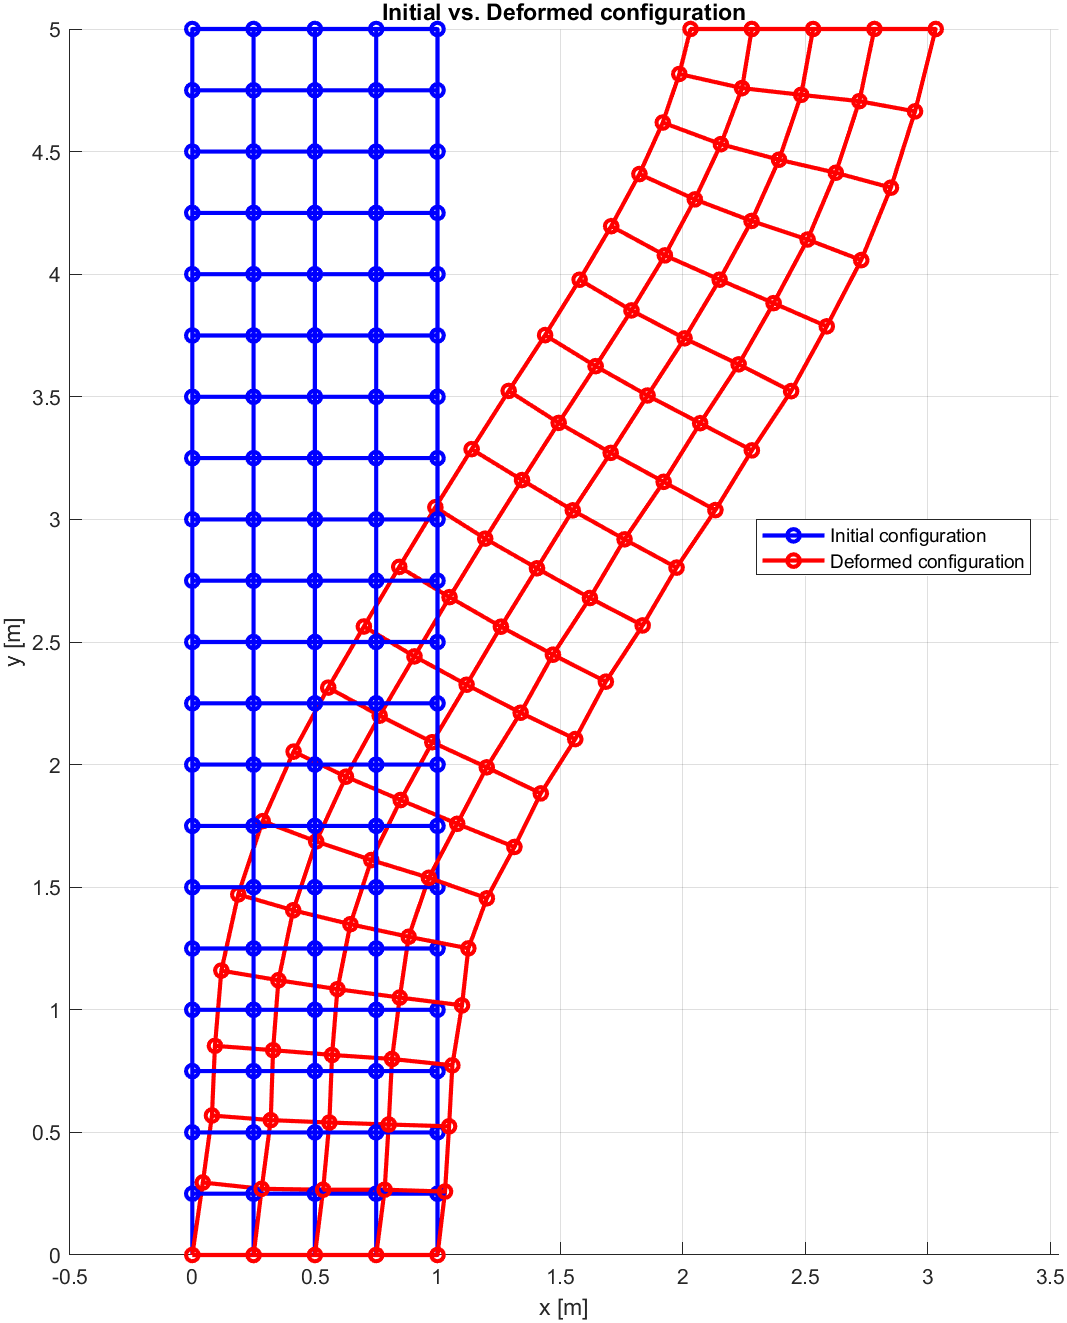
\includegraphics[width=\textwidth]{img/mesh_fine.png}
        \caption{Fine mesh.}
    \end{minipage}

    \caption{Effect of mesh refinement on the results of the simulation.}
    \label{fig:mesh_refinement}

\end{figure}

From Figure \ref{fig:mesh_refinement}, it's clear that the results of the simulation are affected by the choice of the mesh size.
In particular, given the high loading speed and the inertia effects, the results of the simulation are more accurate when a fine mesh is used, where the mass distribution is more accurate.
In the coarse mesh, the mass distribution is not accurate (on the central node an equivalent $25\%$ of the total mass is applied), and the inertia effects are not well represented, leading to a not realistic slow behavior of the node.
